\section{TODO Applying a Gaussian Process to Astrostatistics}
% Possible domains:
% 
% 
% Materials science \cite{materials}
% 
% 
% Cosmography \cite{cosmography}
% 
% 
% Statistical emulators \cite{emulators}
% 
% 
% Signals processing \cite{signals-processing}


\subsection{Introduction}

\subsubsection{Astrological background: SED modelling}
The optical light from a distant galaxy, integrated over its entire size in the sky, comes from stars and gas in the galaxy that shine. We can find the spectral energy distribution (SED) of the galaxy by measuring the brightness at different wavelength bands. Brightness at specific wavelenghts can be used to infer the existence of certain behaviours in the galaxy's gases and stars. 

\begin{figure}[H]
	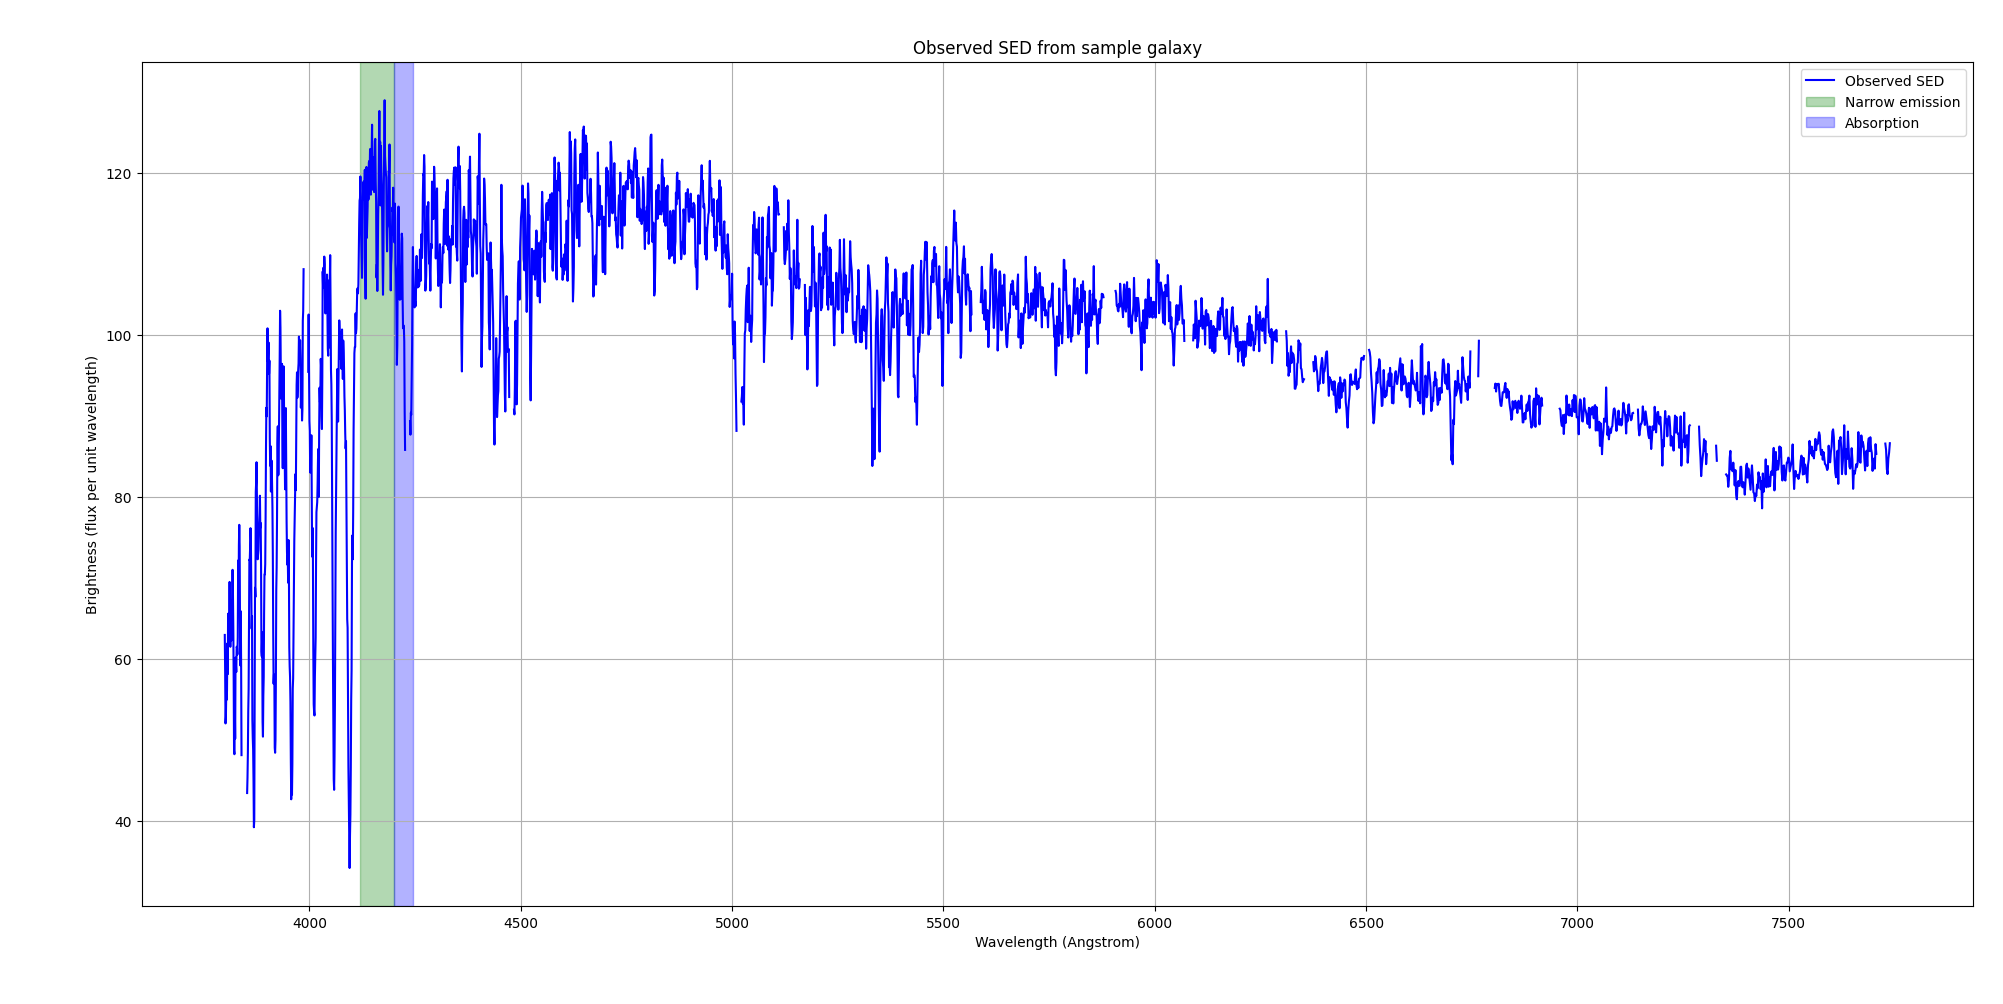
\includegraphics[height=0.5\textwidth]{application/observed-spectrum.png}
    \caption{SED of a sample galaxy (id 51613-0305-552) \cite{galaxy-gp-noise}.
\end{figure}
The 4000-4500 wavelength region of this SED contains two examples of how a galaxy's age can be inferred after observing their SED. The upward narrow emission band highlighted in green is from ionised gas, mostly Hydrogen and Oxygen in this wavelength range, produced by younger stars. The downward dipping absorption band in red is from electronic transitions in the stars atmospheres, such as Hydrogen and Calcium, that occurs in older stars \cite{galaxy-spectra-101}. Astronomers use very complex models with many free parameters and hidden variables to understand the effect of characteristics of the stars and gases of the galaxy on the SED \cite{galaxy-spectra-101}.

\begin{figure}[H]
    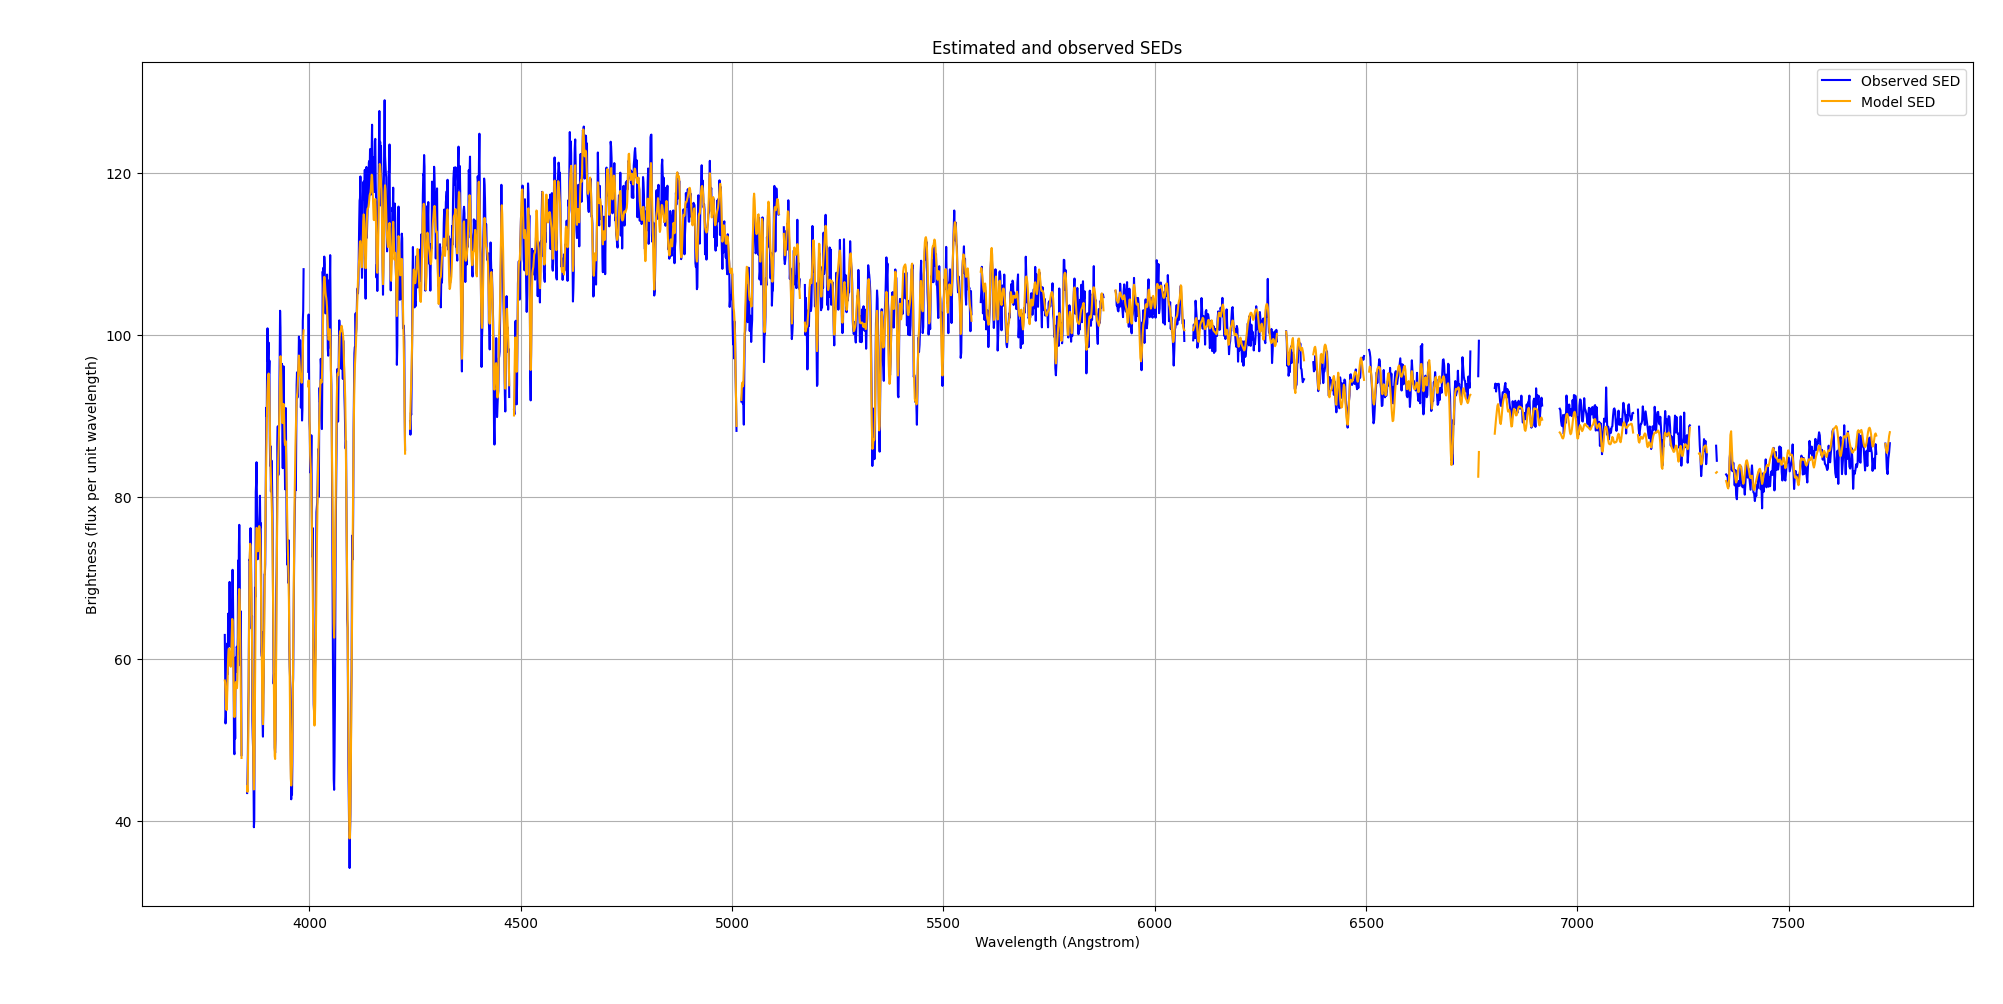
\includegraphics[height=0.5\textwidth]{application/model.png}
    \caption{SED estimated using Leung's model of the the sample galaxy alongside its observed SED \cite{galaxy-gp-noise}.}
\end{figure}
Leung's model \cite{galaxy-gp-noise} agreed with the observed SED in that the regions we identified as emissions and absorption bands but failed to predict brightness in other regions of the SED. In particular, large amounts of true emmissions were missed in a low wavelength region (<4500 Angstroms) and a high wavelength region (6500-7500 Angstroms), while the model predicted a large absorption band in the 4100 Angstrom region that did not exist.

\subsubsection{Low-frequency wobbles}
\begin{figure}[H]
    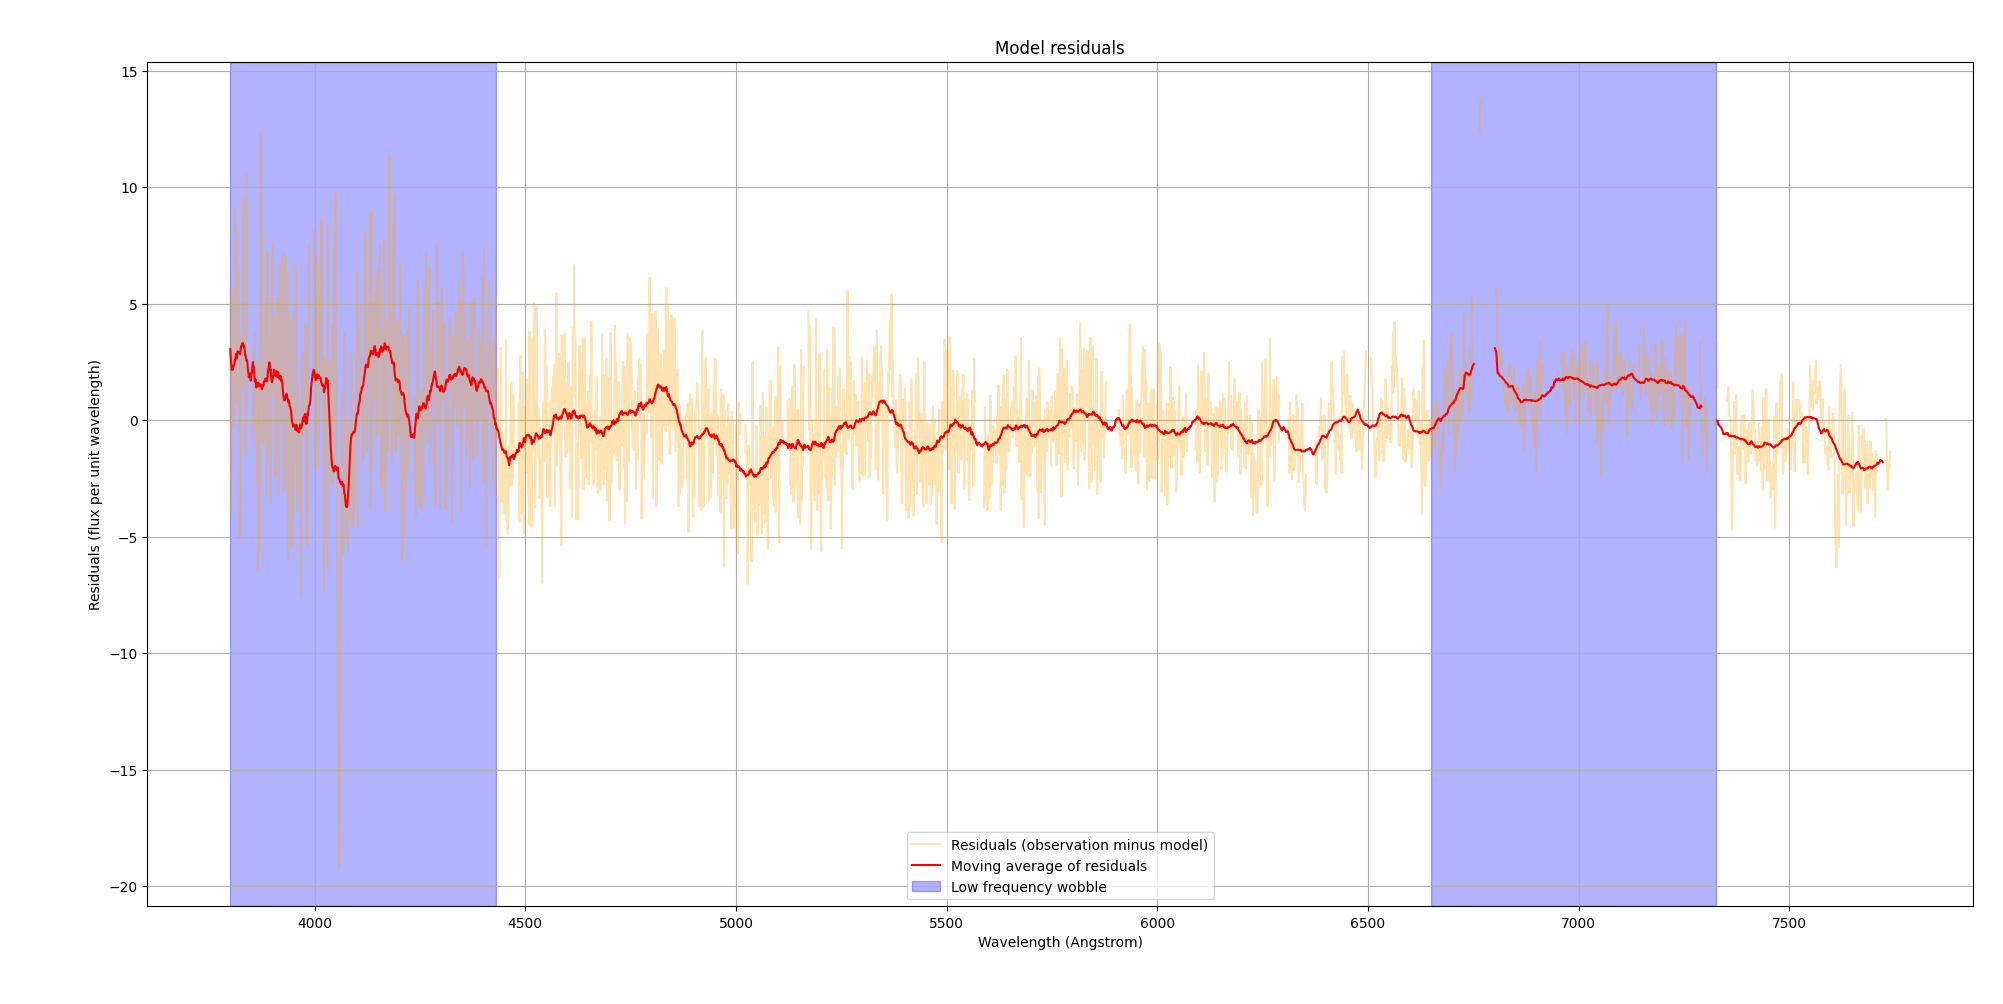
\includegraphics[height=0.5\textwidth]{application/raw_residuals.png}
    \caption{Residuals of the model fit to the SED of the same galaxy \cite{galaxy-gp-noise}.}
\end{figure}
Residuals that behave as zero-mean noise are dependent on how long we observe the galaxy for and are not of interest \cite{galaxy-spectra-101}. However, the two regions identified previously are reflected in the model's residuals - the residuals oscillate above zero in the low and high wavelength regions, with the exception of the 4100 Angstrom region nevative residual spike. We refer to these regions as low frequency wobbles, because these oscillations occur at a lower frequency than the oscillations around zero in the remaining SED. An SED model exhibiting low-frequency wobbles are problematic to use for inference as they violate the zero-mean noise assumption \ref{eq:model_error_assumption}. 

% A low frequency wobble has two sources: problems with the data reduction process, and problems with the model. We can seperate these sources by modelling large numbers of galaxies that differ greatly in their distance to Earth. Light from farther galaxies that takes longer to reach us exhibits is shifted to longer wavelengths - aphenomenon called "redshift",  due to the expansion of the universe. Low frequency wobbles caused by data reduction problems will occur in the same observed wavelength region for all galaxies, while low frequency wobbles caused by the model will occur in different observed wavelength regions \cite{galaxy-spectra-101}.

\subsubsection{Using GPs for SED residual modelling}
SAs the source of low-frequency wobbles is presently not well understood and cannot be incorporated into an SED model \cite{galaxy-spectra-101}, we need a method to remove these low-frequency wobbles without altering or biasing the high-frequency noise that is required for inference (e.g. standard errors in frequentist regression). Signals processing methods that filter out the low-frequency wobble and retain the high-frequency noise would require a fixed frequency cutoff, which does not exist as the amplitude and scale of the low-frequency wobbles vary between galaxies and needs to be learned from the data. Conversly, a neural network trained on thousands of examples of SED residuals would produce point estimates of residuals, the uncertainty of which would be difficult to quantify and propagate. 

\begin{figure}[H]
    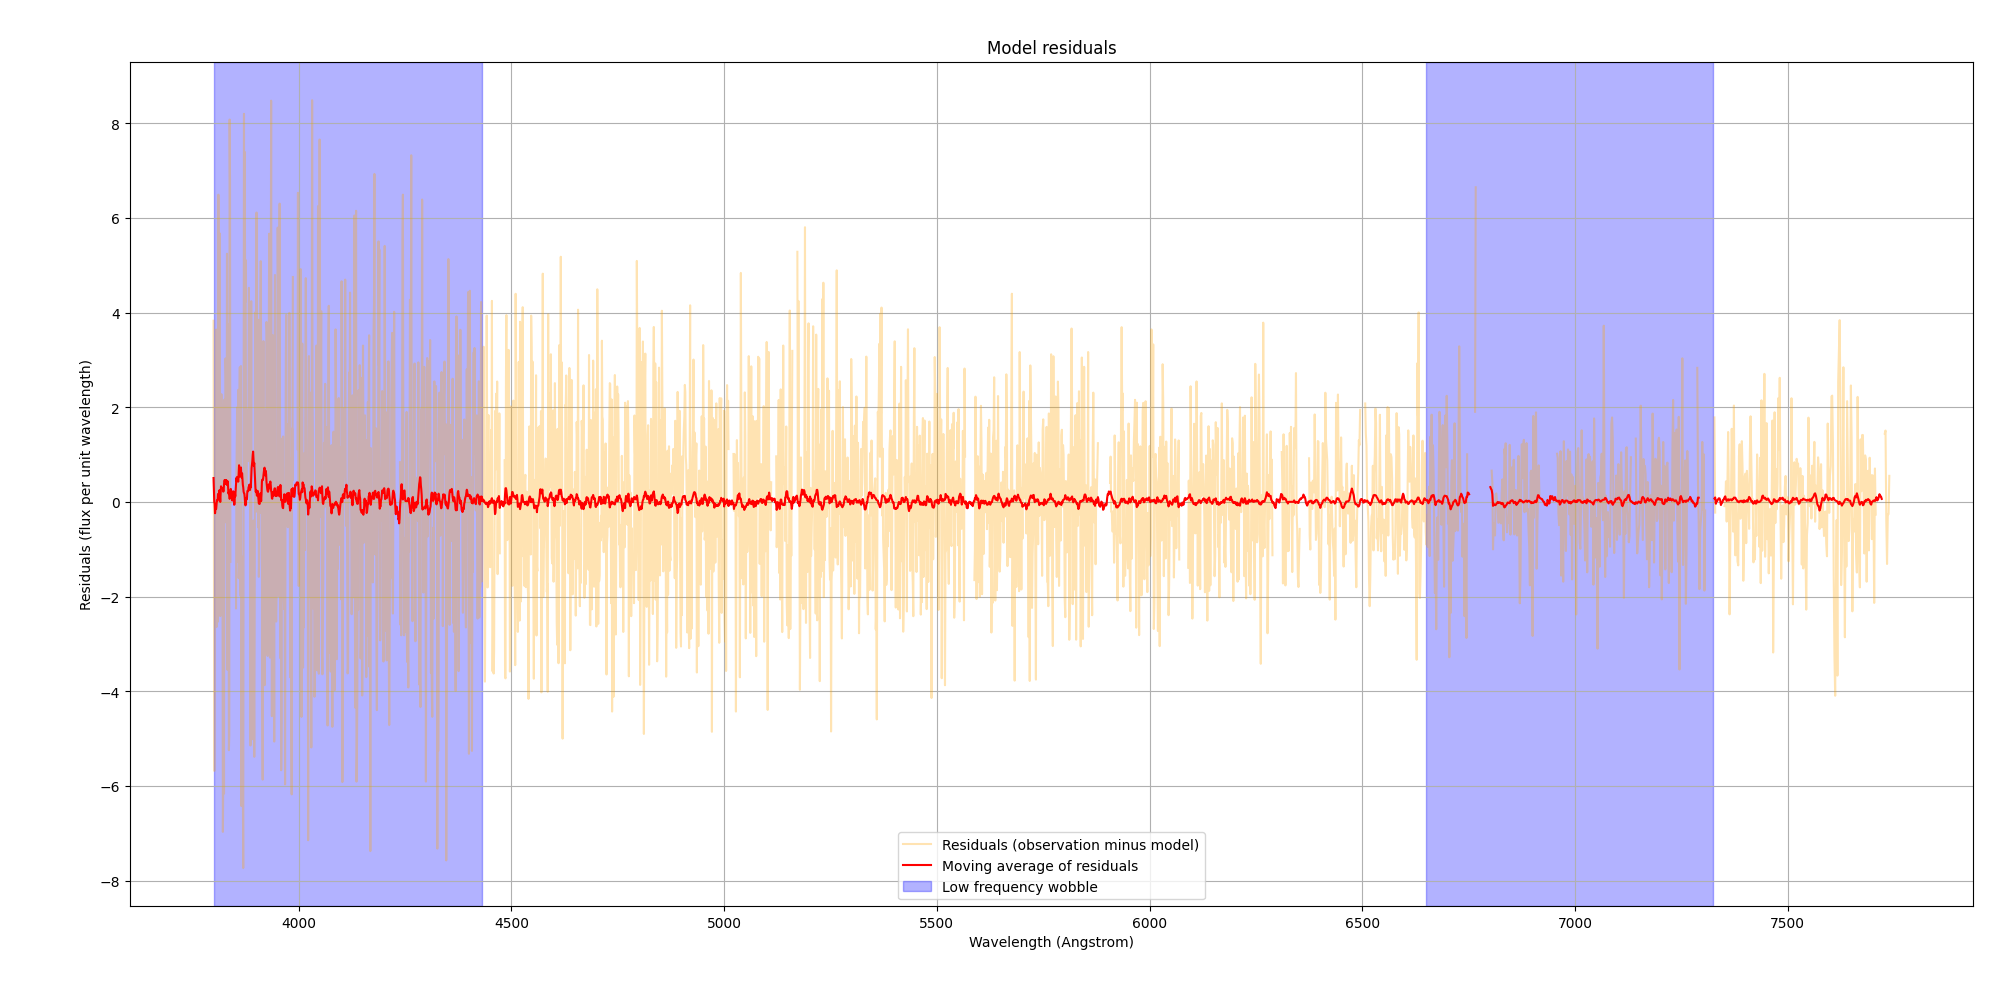
\includegraphics[height=0.5\textwidth]{application/gp_residuals.png}
    \caption{These are the remaining residuals after fitting a GP using SE \cite{galaxy-gp-noise} to the raw residuals of the previous SED model.}
\end{figure}
GPs are a natural choice for this problem as they can identify the low-frequency wobbles on a per-galaxy basis, whilst doing so in a probabilistic framework that allows the uncertainty in this estimation to be properly quantified. SE \ref{eq:se} is a good kernel for SED modelling because its spectral density converges to zero faster than any other kernel, which means it models the low-frequency wobbles whilst ignoring the high-frequency noise. Unfortunately, GPs have a naive training and inference cost of $O(n^3)$ and each SED data contains thousands of data points (e.g. the example galaxy has 3000 data points), which makes training and inference on a single galaxy infeasible. We apply two methods of addressing this cubic complexity to enable the use of GPs for SED residual modelling.

\subsection{Methodology}

\subsubsection{Approximations considered}
SVGP is an approximation-based method that sacrifices accuracy and wall-clock time per epoch, in exchange for lower computational complexity $O(bm^2 + m^3)$ and applicability. Conversly, celerite kernels are a more structured method that cannot be applied everywhere and to every kernel and computationally more complex, but have a lower wall-clock time per epoch and produces near-perfect recreations of the full GP.

This dataset meets all the conditions for celerite models: it is one dimensional, because the only input variable is wavelength, and the data is sorted by wavelength. Unfortunately, celerite kernels can only be used with Matern 3/2 which are not as suitable for SED modelling as SE. Since the choice of kernel does not affect the computational complexity of the GP or training times, we will compare the performance of SVGP with SE and celerite with Matern 3/2, then compare the accuracy of SVGP using SE to the full GP using SE.

\subsubsection{Computational speed}

% https://gpy.readthedocs.io/en/deploy/ \cite{gpy}

% https://celerite2.readthedocs.io/en/latest/ \cite{foreman-mackay}

\subsection{Results}

\subsection{Discussion}

\subsection{Conclusion}

% test local approximations too
